%\documentclass[hyperref={pdfpagelabels=false},slidetop,9pt]{beamer}
\documentclass[slidetop,8pt]{beamer}
\usepackage[T1]{fontenc}
\usepackage[utf8]{inputenc}
\newcommand{\id}{54}
\newcommand{\nom}{Liaisons mécaniques}
\newcommand{\sequence}{04}
\newcommand{\num}{01}
\newcommand{\type}{TP}
\newcommand{\descrip}{Modélisation d'un solide. Comportement des liaisons mécaniques. Modéliser les mécanismes du laboratoire par un schéma cinématique, paramétré.}
\newcommand{\competences}{A3-C4: Analyse d'architecture et de comportement \\ &  Mod1-C1: Isolement d'un solide ou d'un système de solides \\ &  Mod2-C10-1: Modèle de solide indéformable \\ &  Mod2-C11: Modélisation géométrique et cinématique des mouvements entre solides indéformables \\ &  Mod2-C12: Modélisation cinématique des liaisons entre solides \\ &  Mod2-C15: Modélisation des actions mécaniques \\ &  Rés-C6: Utilisation d'un solveur ou d'un logiciel multi physique \\ &  Com1-C1: Différents descripteurs introduits dans le programme \\ &  Com2-C4: Outils de communication}
\newcommand{\nbcomp}{9}
\newcommand{\systemes}{Plateforme Stewart}
\newcommand{\systemessansaccent}{Plateforme Stewart}
\newcommand{\ilot}{2}
\newcommand{\ilotstr}{02}
\newcommand{\dossierilot}{\detokenize{Ilot_02 Plateforme Stewart}}
\newcommand{\imageun}{Plateforme}

\newcommand{\urlsysteme}{\href{https://www.costadoat.fr/systeme/57}{Ressources système}}
\newcommand{\matlabsimscape}{\href{https://github.com/Costadoat/Sciences-Ingenieur/raw/master/Systemes/Plateforme Stewart/Plateforme_Stewart_Simscape.zip}{Modèle Simscape}}
\newcommand{\solidworks}{\href{https://github.com/Costadoat/Sciences-Ingenieur/raw/master/Systemes/Plateforme Stewart/Plateforme_Stewart_Solidworks.zip}{Modèle Solidworks}}
\newcommand{\edrawings}{\href{https://github.com/Costadoat/Sciences-Ingenieur/raw/master/Systemes/Plateforme Stewart/Plateforme_Stewart.EASM}{Modèle eDrawings}}
\newcommand{\test}{Stewart_param1}
\newcommand{\testi}{Stewart_param2}
\newcommand{\testii}{Stewart_param3}
\newcommand{\testiii}{Stewart_param4}
\newcommand{\testiiii}{Stewart_euler}
\usepackage{etex}
\usepackage{tikz}
\usepackage[european]{circuitikz}
\usepackage{pgf}
\usepackage[all]{xy}
\usepackage{pgfpages}
\usepackage{graphbox}
\usepackage{pdfpages}
\usepackage[adobe-utopia]{mathdesign}
\usepackage{ifthen}
\usepackage{cancel}
\usepackage{framed}
\usepackage{subfig}
\usepackage{tabularx}
\usepackage{setspace}
\usepackage{soul}
\usepackage{schemabloc}
\usepackage{eqnarray}
\usepackage[dot, phantomtext]{dashundergaps}
\usepackage{media9}
\usepackage{multimedia}
\usepackage{textcomp}

\author{Renaud Costadoat}
\institute{Lycée Dorian}

\usepackage{multido}
\usepackage{multirow}
\usepackage{multicol} % Portions de texte en colonnes
\usepackage{flafter}%floatants après la référence

\usepackage{color}
\usepackage{xcolor}
\usepackage{colortbl}

\usepackage[gen]{eurosym}
\usepackage{tikz}
%\usepackage{pstricks,pst-node,pst-tree,pst-solides3d}
\usepackage{lmodern}
\usepackage[francais]{babel}
\usepackage{pslatex}
\usetheme{renaud}
\usepackage{times}
\usepackage{amsmath}
\usepackage{verbatim}
\usepackage{moreverb}
%\usetikzlibrary{arrows,shapes}
\usepackage{graphicx}
\usepackage{psfrag}
\usepackage{wrapfig}
\usepackage{etoolbox}

\definecolor{gris25}{gray}{0.75}
\definecolor{bleu}{RGB}{18,33,98}
\definecolor{bleuf}{RGB}{42,94,171}
\definecolor{bleuc}{RGB}{231,239,247}
\definecolor{rougef}{RGB}{185,18,27}
\definecolor{rougec}{RGB}{255,188,204}%255,230,231
\definecolor{vertf}{RGB}{103,126,82}
\definecolor{vertc}{RGB}{220,255,191}

\setlength\parindent{24pt}
\parskip 7.2pt
\parindent 8pt

\newenvironment{rem}[1][\hsize]%
{%
    \def\FrameCommand
   {%
\rotatebox{90}{\textit{\textsf{Remarque}}} 
       {\color{bleuf}\vrule width 3pt}%
       \hspace{0pt}%must no space.
       \fboxsep=\FrameSep\colorbox{bleuc}%
  }%
    \MakeFramed{\hsize#1\advance\hsize-\width\FrameRestore}%
}%
{\endMakeFramed}%


\newenvironment{savoir}[1][\hsize]%
{%
    \def\FrameCommand
    {%
\rotatebox{90}{\textit{\textsf{Savoir}}} 
        {\color{bleuf}\vrule width 3pt}%
        \hspace{0pt}%must no space.
        \fboxsep=\FrameSep\colorbox{bleuc}%
    }%
    \MakeFramed{\hsize#1\advance\hsize-\width\FrameRestore}%
}%
{\endMakeFramed}%

\newenvironment{prob}[1][\hsize]%
{%
    \def\FrameCommand%
    {%
\rotatebox{90}{\textit{\textsf{Problematique}}} 
        {\color{rougef}\vrule width 3pt}%
        \hspace{0pt}%must no space.
        \fboxsep=\FrameSep\colorbox{rougec}%
    }%
    \MakeFramed{\hsize#1\advance\hsize-\width\FrameRestore}%
}%
{\endMakeFramed}%

\newenvironment{obj}[1][\hsize]%
{%
    \def\FrameCommand%
    {%
\rotatebox{90}{\textit{\textsf{Objectif}}} 
        {\color{vertf}\vrule width 3pt}%
        \hspace{0pt}%must no space.
        \fboxsep=\FrameSep\colorbox{vertc}%
    }%
    \MakeFramed{\hsize#1\advance\hsize-\width\FrameRestore}%
}%
{\endMakeFramed}%

\newenvironment{defi}[1][\hsize]%
{%
    \def\FrameCommand%
    {%
\rotatebox{90}{\textit{\textsf{Definition}}} 
        {\color{bleuf}\vrule width 3pt}%
        \hspace{0pt}%must no space.
        \fboxsep=\FrameSep\colorbox{rougec}%
    }%
    \MakeFramed{\hsize#1\advance\hsize-\width\FrameRestore}%
}%
{\endMakeFramed}%


\newenvironment{hypo}[1][\hsize]%
{%
    \def\FrameCommand%
    {%
\rotatebox{90}{\textit{\textsf{Hypothèse\\}}} 
        {\color{bleuf}\vrule width 3pt}%
        \hspace{0pt}%must no space.
        \fboxsep=\FrameSep\colorbox{bleuc}%
    }%
    \MakeFramed{\hsize#1\advance\hsize-\width\FrameRestore}%
}%
{\endMakeFramed}%


\newenvironment{prop}[1][\hsize]%
{%
    \def\FrameCommand%
    {%
\rotatebox{90}{\textit{\textsf{Propriété}}} 
        {\color{bleuf}\vrule width 3pt}%
        \hspace{0pt}%must no space.
        \fboxsep=\FrameSep\colorbox{bleuc}%
    }%
    \MakeFramed{\hsize#1\advance\hsize-\width\FrameRestore}%
}%
{\endMakeFramed}%

\newenvironment{props}[1][\hsize]%
{%
    \def\FrameCommand%
    {%
\rotatebox{90}{\textit{\textsf{Propriétés}}} 
        {\color{bleuf}\vrule width 3pt}%
        \hspace{0pt}%must no space.
        \fboxsep=\FrameSep\colorbox{bleuc}%
    }%
    \MakeFramed{\hsize#1\advance\hsize-\width\FrameRestore}%
}%
{\endMakeFramed}%

\newenvironment{exemple}[1][\hsize]%
{%
    \def\FrameCommand%
    {%
\rotatebox{90}{\textit{\textsf{Exemple}}} 
        {\color{vertf}\vrule width 3pt}%
        \hspace{0pt}%must no space.
        \fboxsep=\FrameSep\colorbox{vertc}%
    }%
    \MakeFramed{\hsize#1\advance\hsize-\width\FrameRestore}%
}%
{\endMakeFramed}%

\newenvironment{resultat}[1][\hsize]%
{%
    \def\FrameCommand%
    {%
\rotatebox{90}{\textit{\textsf{Résultat}}} 
        {\color{rougef}\vrule width 3pt}%
%        {\color{bleuf}\vrule width 3pt}%
        \hspace{0pt}%must no space.
        \fboxsep=\FrameSep\colorbox{rougec}%
    }%
    \MakeFramed{\hsize#1\advance\hsize-\width\FrameRestore}%
}%
{\endMakeFramed}%

\newenvironment{methode}[1][\hsize]%
{%
    \def\FrameCommand%
    {%
\rotatebox{90}{\textit{\textsf{Méthode\\}}} 
        {\color{rougef}\vrule width 3pt}%
        \hspace{0pt}%must no space.
        \fboxsep=\FrameSep\colorbox{rougec}%
    }%
    \MakeFramed{\hsize#1\advance\hsize-\width\FrameRestore}%
}%
{\endMakeFramed}%

\newenvironment{theo}[1][\hsize]%
{%
    \def\FrameCommand%
    {%
\rotatebox{90}{\textit{\textsf{Théorème\\}}} 
        {\color{rougef}\vrule width 3pt}%
        \hspace{0pt}%must no space.
        \fboxsep=\FrameSep\colorbox{rougec}%
    }%
    \MakeFramed{\hsize#1\advance\hsize-\width\FrameRestore}%
}%
{\endMakeFramed}%

\newenvironment{warn}[1][\hsize]%
{%
    \def\FrameCommand%
    {%
\rotatebox{90}{\textit{\textsf{Attention\\}}} 
        {\color{rougef}\vrule width 3pt}%
        \hspace{0pt}%must no space.
        \fboxsep=\FrameSep\colorbox{rougec}%
    }%
    \MakeFramed{\hsize#1\advance\hsize-\width\FrameRestore}%
}%
{\endMakeFramed}%

% \usepackage{pstricks}
%\usepackage{minitoc}
% \setcounter{minitocdepth}{4}

\setcounter{tocdepth}{2}

% \mtcselectlanguage{french} 

%\usepackage{draftcopy}% "Brouillon"
% \usepackage{floatflt}
\usepackage{psfrag}
%\usepackage{listings} % Permet d'insérer du code de programmation
\renewcommand{\baselinestretch}{1.2}

% Changer la num�rotation des figures :
% ------------------------------------
% \makeatletter
% \renewcommand{\thefigure}{\ifnum \c@section>\z@ \thesection.\fi
%  \@arabic\c@figure}
% \@addtoreset{figure}{section}
% \makeatother
 


%%%%%%%%%%%%
% Définition des vecteurs %
%%%%%%%%%%%%
 \newcommand{\vect}[1]{\overrightarrow{#1}}

%%%%%%%%%%%%
% Définition des torseusr %
%%%%%%%%%%%%

 \newcommand{\torseur}[1]{%
\left\{{#1}\right\}
}

\newcommand{\torseurcin}[3]{%
\left\{\mathcal{#1} \left(#2/#3 \right) \right\}
}

\newcommand{\torseurstat}[3]{%
\left\{\mathcal{#1} \left(#2\rightarrow #3 \right) \right\}
}

 \newcommand{\torseurc}[8]{%
%\left\{#1 \right\}=
\left\{
{#1}
\right\}
 = 
\left\{%
\begin{array}{cc}%
{#2} & {#5}\\%
{#3} & {#6}\\%
{#4} & {#7}\\%
\end{array}%
\right\}_{#8}%
}

 \newcommand{\torseurcol}[7]{
\left\{%
\begin{array}{cc}%
{#1} & {#4}\\%
{#2} & {#5}\\%
{#3} & {#6}\\%
\end{array}%
\right\}_{#7}%
}

 \newcommand{\torseurl}[3]{%
%\left\{\mathcal{#1}\right\}_{#2}=%
\left\{%
\begin{array}{l}%
{#1} \\%
{#2} %
\end{array}%
\right\}_{#3}%
}

 \newcommand{\vectv}[3]{%
\vect{V\left( {#1} \in {#2}/{#3}\right)}
}


\newcommand{\vectf}[2]{%
\vect{R\left( {#1} \rightarrow {#2}\right)}
}

\newcommand{\vectm}[3]{%
\vect{\mathcal{M}\left( {#1}, {#2} \rightarrow {#3}\right)}
}


 \newcommand{\vectg}[3]{%
\vect{\Gamma \left( {#1} \in {#2}/{#3}\right)}
}

 \newcommand{\vecto}[2]{%
\vect{\Omega\left( {#1}/{#2}\right)}
}

\newcommand{\reponse}[1][4]
{
\multido{}{#1}
{
\begin{center}
\makebox[0.9\linewidth]{\dotfill} \end{center}
}}


% }$$\left\{\mathcal{#1} \right\}_{#2} =%
% \left\{%
% \begin{array}{c}%
%  #3 \\%
%  #4 %
% \end{array}%
% \right\}_{#5}}


%  ------------------------------------------
% | Modification du formatage des sections : | 
%  ------------------------------------------

% Grands titres :
% ---------------

\newcommand{\titre}[1]{%
\begin{center}
      \bigskip
      \rule{\textwidth}{1pt}
      \par\vspace{0.1cm}
      
      \textbf{\large #1}
      \par\rule{\textwidth}{1pt}
    \end{center}
    \bigskip
  }

% Supprime le numéro du chapitre dans la numérotation des sections:
% -----------------------------------------------------------------
\makeatletter
\renewcommand{\thesection}{\@arabic\c@section}
\makeatother


% \titleformat{\chapter}[display]
% {\normalfont\Large\filcenter}
% {}
% {1pc}
% {\titlerule[1pt]
%   \vspace{1pc}%
%   \Huge}[\vspace{1ex}%
% \titlerule]


%%%% Chapitres Comme PY Pechard %%%%%%%%%
% numéro du chapitre
\DeclareFixedFont{\chapnumfont}{OT1}{phv}{b}{n}{80pt}
% pour le mot " Chapitre "
\DeclareFixedFont{\chapchapfont}{OT1}{phv}{m}{it}{40pt}
% pour le titre
\DeclareFixedFont{\chaptitfont}{T1}{phv}{b}{n}{25pt}

\definecolor{gris}{gray}{0.75}
\setbeamertemplate{section in toc}[sections numbered]

\newlength{\RoundedBoxWidth}
\newsavebox{\GrayRoundedBox}
\newenvironment{GrayBox}[1][\dimexpr\textwidth-4.5ex]%
   {\setlength{\RoundedBoxWidth}{\dimexpr#1}
    \begin{lrbox}{\GrayRoundedBox}
       \begin{minipage}{\RoundedBoxWidth}}%
   {   \end{minipage}
    \end{lrbox}
    \begin{center}
    \begin{tikzpicture}%
       \draw node[draw=bleuf,fill=bleuc,rounded corners,%
             inner sep=2ex,text width=\RoundedBoxWidth]%
             {\usebox{\GrayRoundedBox}};
    \end{tikzpicture}
    \end{center}}
    
\ifdef{\prive}{\pgfpagesuselayout{2 on 1}[a4paper,border shrink=0mm]}
\ifdef{\prive}{\setbeamertemplate{navigation symbols}{}}
\setbeamertemplate{itemize item}[ball]
%\setbeamertemplate{blocks}[rounded]%[shadow=true]
\setbeamercolor{block title}{fg=white,bg=grisf}        % titre block normal 
\setbeamercolor{block body}{fg=grisf,bg=grisc!50}      % corps block normal
\setbeamercolor{block body alerted}{fg=white,bg=warning}   % idem pour un block alerte

\title{\nom}
\date{S\sequence \ - \type\num}

\begin{document}
\shorthandoff{:!}
\bibliographystyle{abbrvnat-fr}

\usebackgroundtemplate%
{%
    \centering
\includegraphics[width=\paperwidth]{../../img/fond2}%
}

{
\setbeamertemplate{navigation symbols}{}
\setbeamertemplate{headline}[pagetitre]
\setbeamertemplate{footline}[pagetitre]
\usebackgroundtemplate{\centering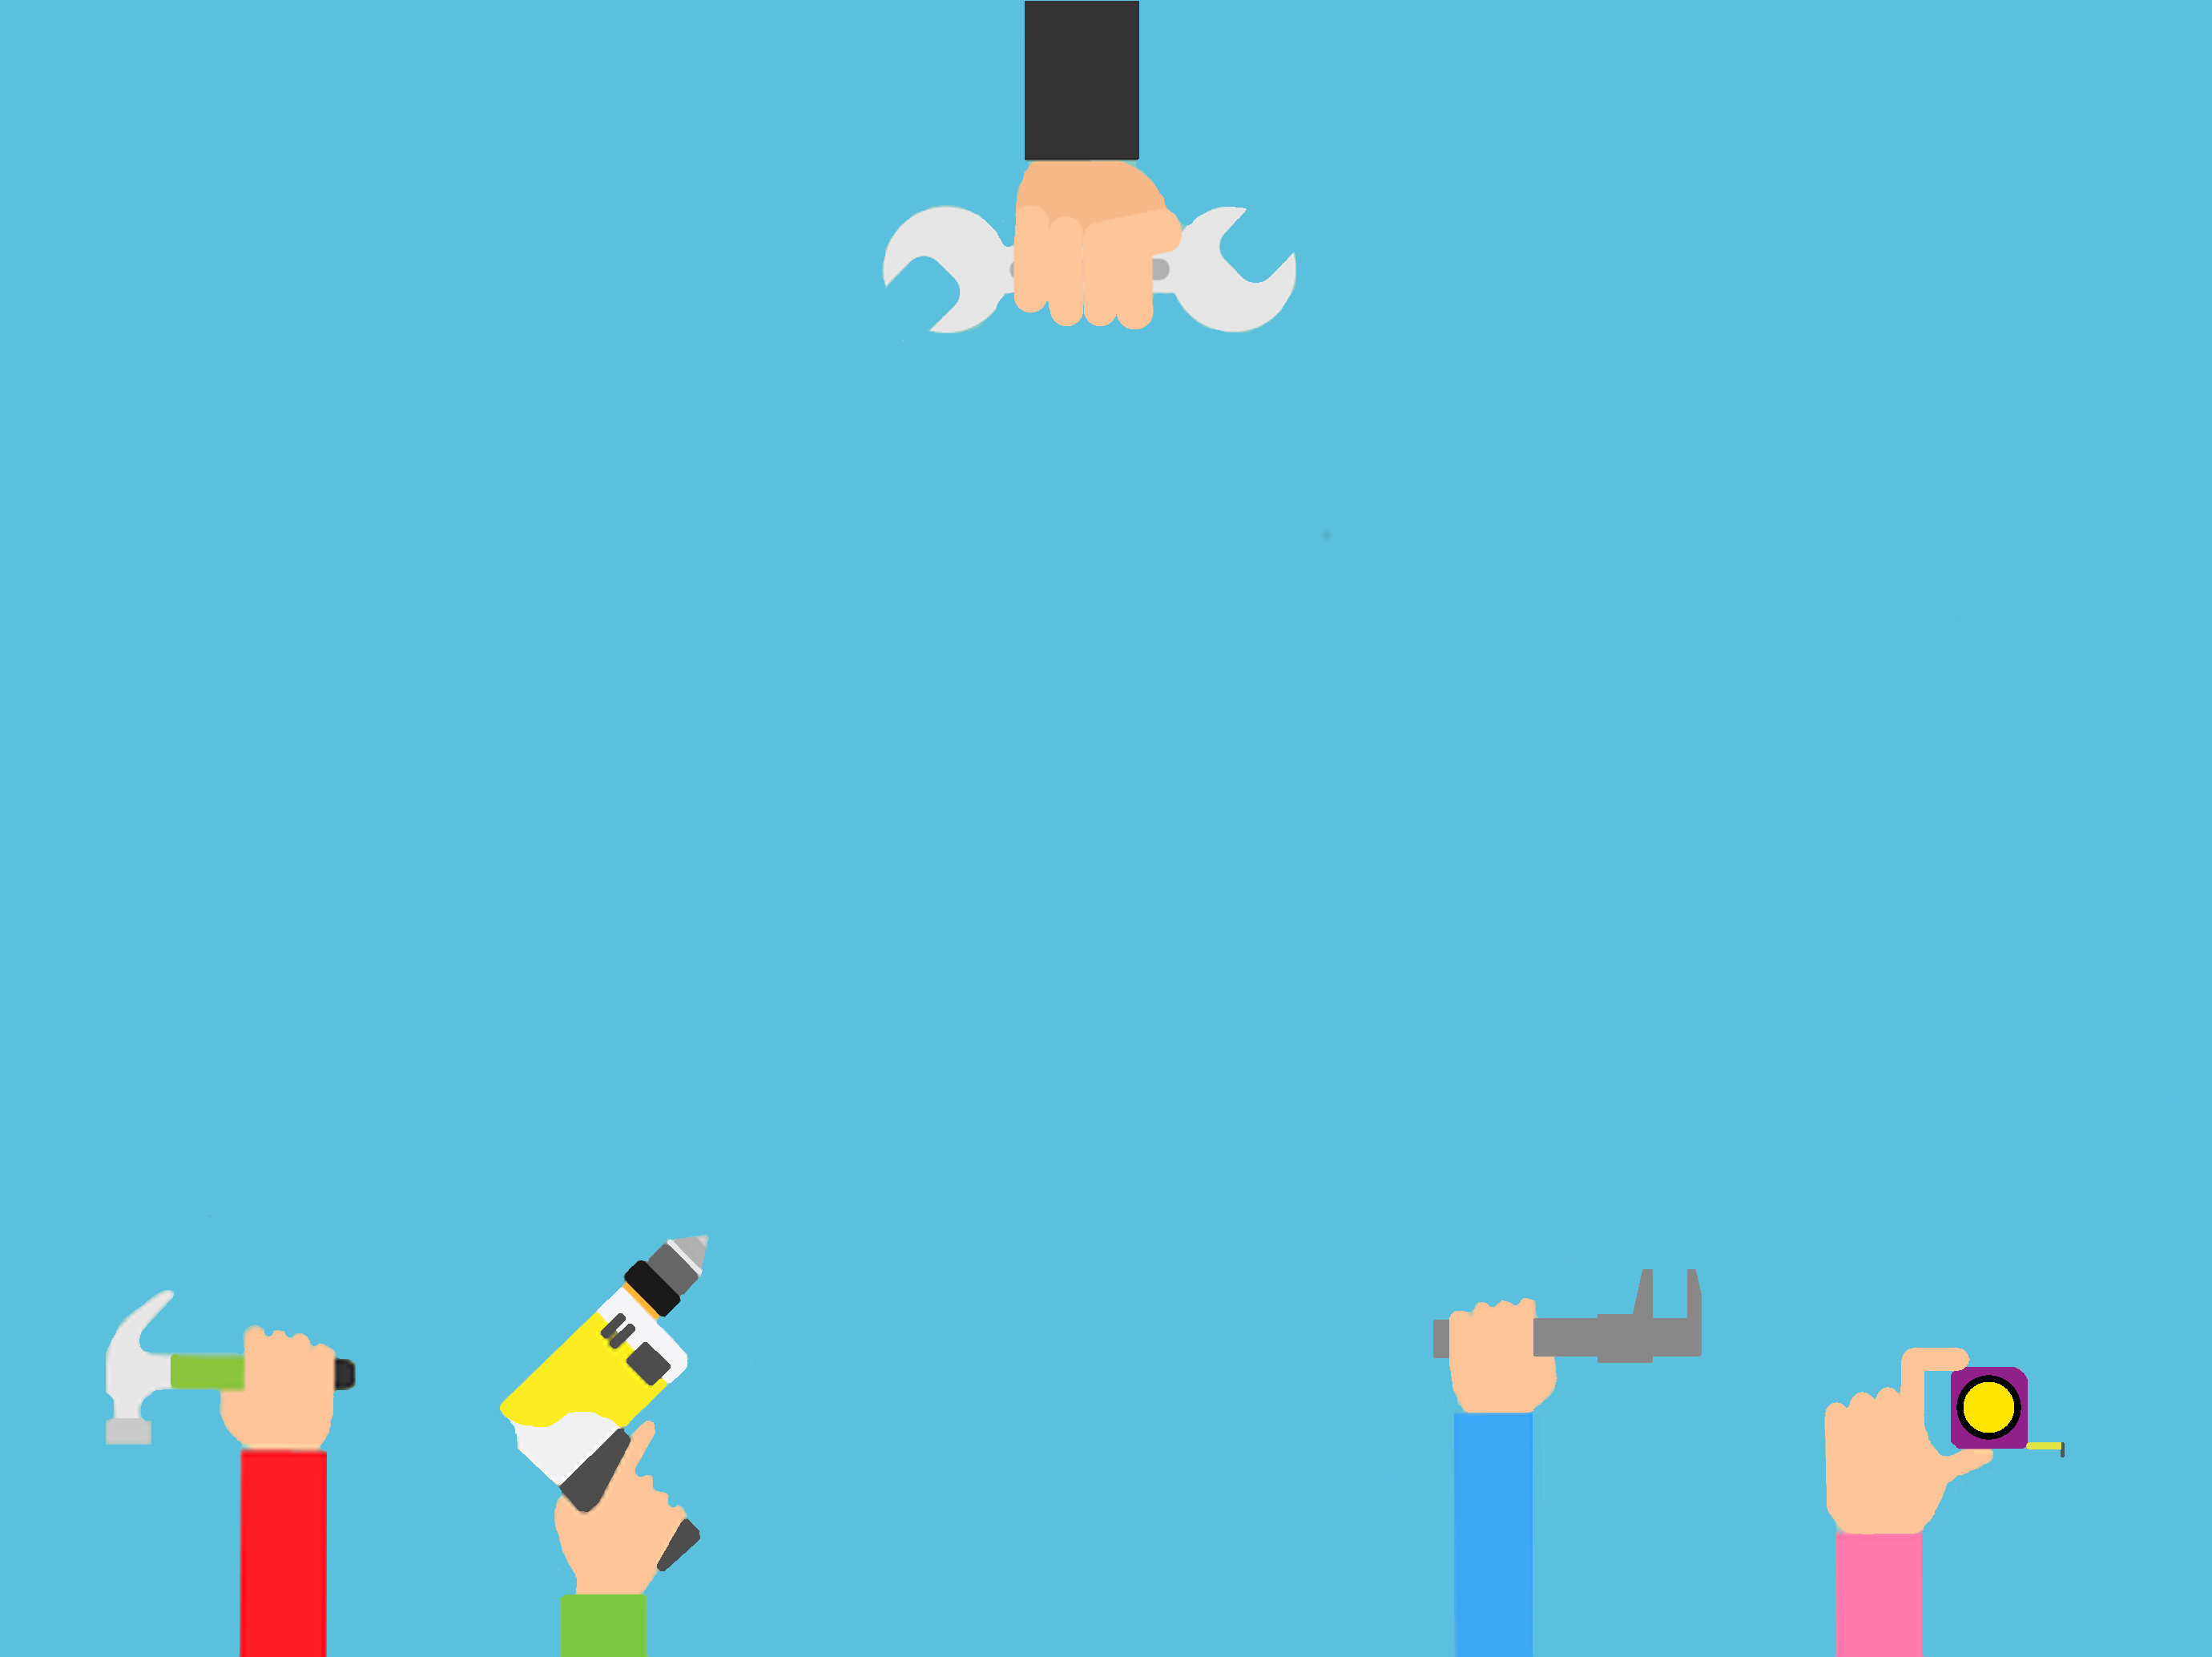
\includegraphics[width=\paperwidth]{../../img/fond}}
\frame{\titlepage}
}




{\frame{
\frametitle{Introduction}

\begin{savoir}
Vous êtes capables :
\begin{itemize}
 \item de donner certaines caractéristiques d'un matériau,
 \item de choisir un procédé de mise en forme de pièces brutes.
\end{itemize}
\end{savoir}

\begin{prob}
Vous devez êtes capables de choisir un procédé d'usinage en fonction:
\begin{itemize}
 \item de la géométrie d'une pièce,
 \item de son matériau,
 \item de la production associée à la pièce.
\end{itemize}
\end{prob}
}}

\section{Moyens de production}

\ifdef{\public}{{\frame{
\frametitle{Plan}
  \tableofcontents[currentsection]
}}}

{\frame{
\frametitle{Les différents types de machine}

L'atelier d'usinage est composé de plusieurs pôles. Chaque pôle dispose du même type de machine, par exemple :
\begin{itemize}
 \item Tour conventionnel,
 \item Fraiseuse conventionnelle,
 \item Tour à commande numérique,
 \item Fraiseuse à commande numérique.
\end{itemize}
}}

{\frame{
\frametitle{Tour}

\begin{itemize}
 \item Cette machine sert principalement à usiner des pièces de révolution. La pièce est fixée dans le mandrin. \\
 \begin{minipage}{0.45\linewidth}
 \item Celui-ci est mis en rotation par le moteur de broche. L'outil suit une trajectoire qui interfère avec la pièce. L'outil est muni d'une arête coupante, il en résulte un enlèvement de matière : les copeaux.
 \end{minipage}\hfill
 \begin{minipage}{0.5\linewidth}
  \centering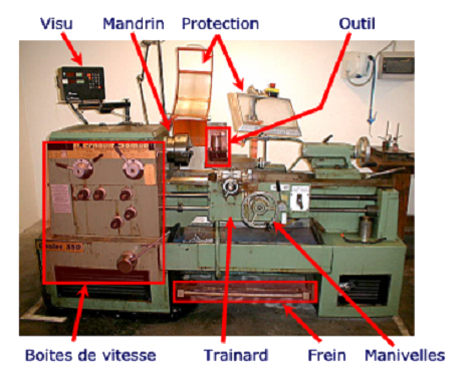
\includegraphics[width=0.9\linewidth]{img/Picture1}
 \end{minipage}
\end{itemize}
}}

{\frame{
\frametitle{Fraiseuse}

\begin{itemize}
\begin{minipage}{0.45\linewidth}
 \item Cette machine sert principalement à usiner des pièces prismatiques. La pièce est fixée dans l'étau,
 \item L'outil est mis en rotation par le moteur de broche, il suit une trajectoire qui interfère avec la pièce.
 \end{minipage}\hfill
 \begin{minipage}{0.5\linewidth}
  \centering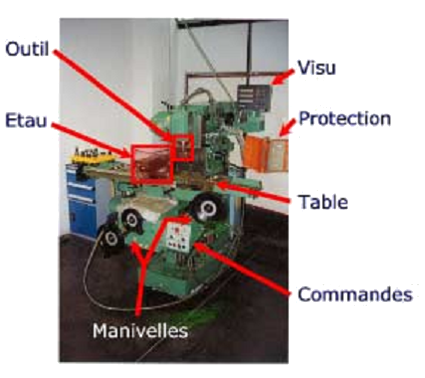
\includegraphics[width=0.9\linewidth]{img/Picture2}
 \end{minipage}
\end{itemize}
}}

{\frame{
\frametitle{Type de commande}

\begin{minipage}[t]{0.45\linewidth}
\textbf{Manuelle ou conventionnelle:}\\ Le déplacement de l'outil sur la trajectoire d'usinage est réalisé par un opérateur. Pour cela, il utilise les manivelles permettant de générer les mouvements suivant les axes. \\ ~\ \\
  \begin{center}
  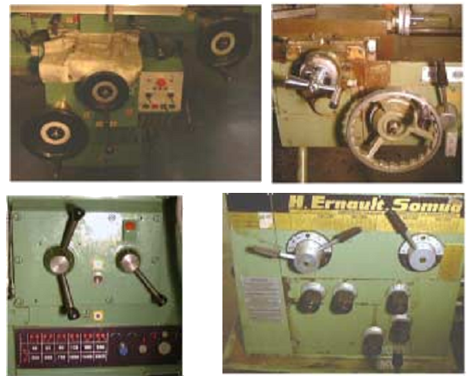
\includegraphics[width=0.9\linewidth]{img/Picture3}
  \end{center}
\end{minipage}\hfill
\begin{minipage}[t]{0.45\linewidth}
\textbf{Commande numérique:} \\ Le déplacement de l'outil sur la trajectoire d'usinage est décrit par l'opérateur à l'aide d'un programme. On utilise pour cela les coordonnées des différents points de passage de l'outil par rapport à la pièce. \\ ~\ \\
   \begin{center}
  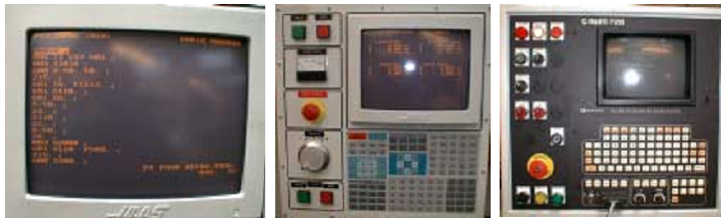
\includegraphics[width=0.9\linewidth]{img/Picture4}
  \end{center}
\end{minipage}
}}

{\frame{
\frametitle{Les axes de déplacements : Tournage}
\begin{itemize}
 \item Afin de décrire la trajectoire suivi par l'outil pour usiner la pièce, un système d'axe est normalisé. En tournage, l'axe de broche correspond à l'axe de rotation de la pièce,
 \item L'axe Z correspond à l'axe de broche. C'est aussi l'axe de rotation du mandrin,
 \item L'axe X correspond à l'axe perpendiculaire à Z. (+ l'outil s'éloigne de la pièce).
\end{itemize}

   \begin{center}
  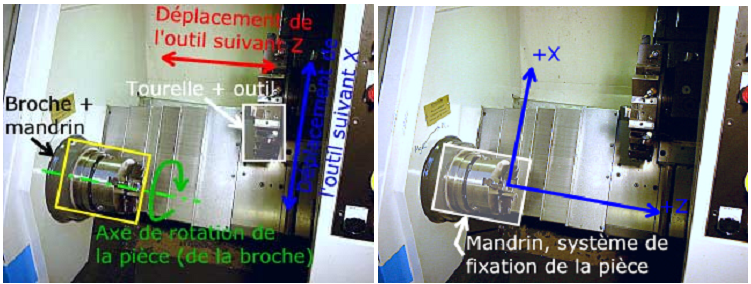
\includegraphics[width=0.9\linewidth]{img/Picture5}
  \end{center}
}}

{\frame{
\frametitle{Les axes de déplacements : Fraisage}
\begin{itemize}
 \item L'axe Z correspond à l'axe de broche. C'est l'axe de rotation de la fraise pour l'usinage,
 \item L'axe X correspond à l'axe perpendiculaire à Z qui permet le plus grand déplacement de la table de la fraiseuse. (+ l'outil s'éloigne de la pièce),
 \item L'axe Y correspond à l'axe perpendiculaire à Z et X. 
\end{itemize}

   \begin{center}
  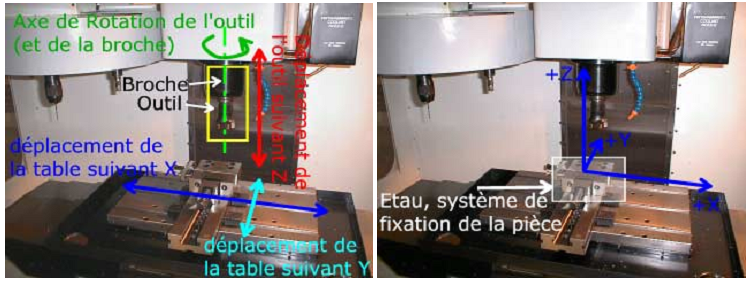
\includegraphics[width=0.9\linewidth]{img/Picture6}
  \end{center}
}}


\section{Géométrie issues de l'usinage}

\ifdef{\public}{{\frame{
\frametitle{Plan}
  \tableofcontents[currentsection]
}}}

{\frame{
\frametitle{Formes simples usinables: Tournage}

\begin{itemize}
\begin{minipage}{0.7\linewidth}
 \item \textbf{Dressage} : C'est la réalisation d'un plan perpendiculaire à l'axe de la pièce  (surface rouge),
 \item \textbf{Chariotage} : C'est la réalisation d'un cylindre ayant le même axe que celui de la pièce (surface grise),
 \item \textbf{Plan épaulé} : C'est l'association d'un dressage et d'un chariotage (surface verte).
\end{minipage}\hfill
\begin{minipage}{0.25\linewidth}
   \begin{center}
  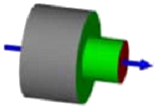
\includegraphics[width=0.8\linewidth]{img/Picture7}
  \end{center}
\end{minipage}\\ ~\ \\
\begin{minipage}{0.55\linewidth}
 \item \textbf{Perçage} : C'est un trou dans la pièce. Il peut être débouchant ou  borgne. Attention en tournage, l'axe du trou est confondu  avec l'axe de la pièce,
\end{minipage}\hfill
\begin{minipage}{0.4\linewidth}
   \begin{center}
  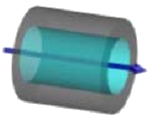
\includegraphics[width=0.4\linewidth]{img/Picture8}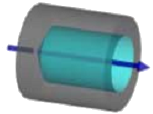
\includegraphics[width=0.4\linewidth]{img/Picture9}
  \end{center}
\end{minipage}\\ ~\ \\
\begin{minipage}{0.55\linewidth}
 \item \textbf{Gorge} : C'est l'association de 2 plans parallèles avec un cylindre (surface vertes),
\end{minipage}\hfill
\begin{minipage}{0.4\linewidth}
   \begin{center}
  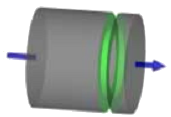
\includegraphics[width=0.45\linewidth]{img/Picture10}
  \end{center}
\end{minipage}\\ ~\ \\
\begin{minipage}{0.55\linewidth}
 \item \textbf{Quelconque} : C'est l'association de plusieurs surfaces élémentaires : 
sphère, cylindre, plan, cône,
\end{minipage}\hfill
\begin{minipage}{0.4\linewidth}
   \begin{center}
  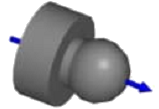
\includegraphics[width=0.45\linewidth]{img/Picture11}
  \end{center}
\end{minipage}
\end{itemize}
}}

{\frame{
\frametitle{Formes simples usinables: Fraisage}

\begin{itemize}
\begin{minipage}{0.7\linewidth}
 \item \textbf{Surfaçage} : Le surfaçage c'est l'usinage d'un plan par une fraise. (surface rouge),
\end{minipage}\hfill
\begin{minipage}{0.25\linewidth}
   \begin{center}
  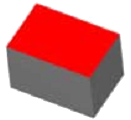
\includegraphics[width=0.6\linewidth]{img/Picture12}
  \end{center}
\end{minipage}\\ ~\ \\
\begin{minipage}{0.7\linewidth}
 \item \textbf{Plans épaulés} : C'est l'association de 2 plans perpendiculaires (surfaces vertes),
\end{minipage}\hfill
\begin{minipage}{0.25\linewidth}
   \begin{center}
  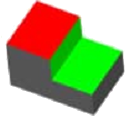
\includegraphics[width=0.6\linewidth]{img/Picture13}
  \end{center}
\end{minipage}\\ ~\ \\
\begin{minipage}{0.7\linewidth}
 \item \textbf{Rainure} : C'est l'association de 3 plans. Le fond est perpendiculaire au deux autres plans. (surfaces vertes),
\end{minipage}\hfill
\begin{minipage}{0.25\linewidth}
   \begin{center}
  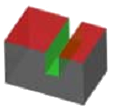
\includegraphics[width=0.6\linewidth]{img/Picture14}
  \end{center}
\end{minipage}\\ ~\ \\
\begin{minipage}{0.7\linewidth}
 \item \textbf{Poche} : La poche est délimitée par des surfaces verticales quelconque (cylindre et plan). C'est une forme creuse dans la pièce. (surface cyan),
\end{minipage}\hfill
\begin{minipage}{0.25\linewidth}
   \begin{center}
  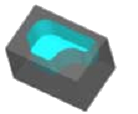
\includegraphics[width=0.6\linewidth]{img/Picture15}
  \end{center}
\end{minipage}\\ ~\ \\
\begin{minipage}{0.7\linewidth}
 \item \textbf{Perçage} : Ce sont des trous. Ils sont débouchants (surface bleu) ou borgnes (surface jaune).
\end{minipage}\hfill
\begin{minipage}{0.25\linewidth}
   \begin{center}
  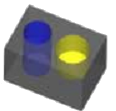
\includegraphics[width=0.6\linewidth]{img/Picture16}
  \end{center}
\end{minipage}
\end{itemize}
}}

\section{Outils}

\ifdef{\public}{{\frame{
\frametitle{Plan}
  \tableofcontents[currentsection]
}}}

{\frame{
\frametitle{Outils de perçage}

\begin{center}
 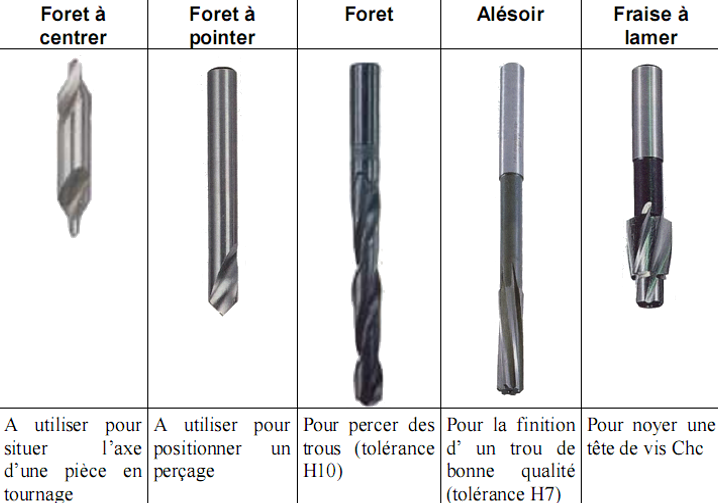
\includegraphics[width=0.8\linewidth]{img/Picture17}
\end{center}

}}

{\frame{
\frametitle{Outils de tournage}

\begin{center}
 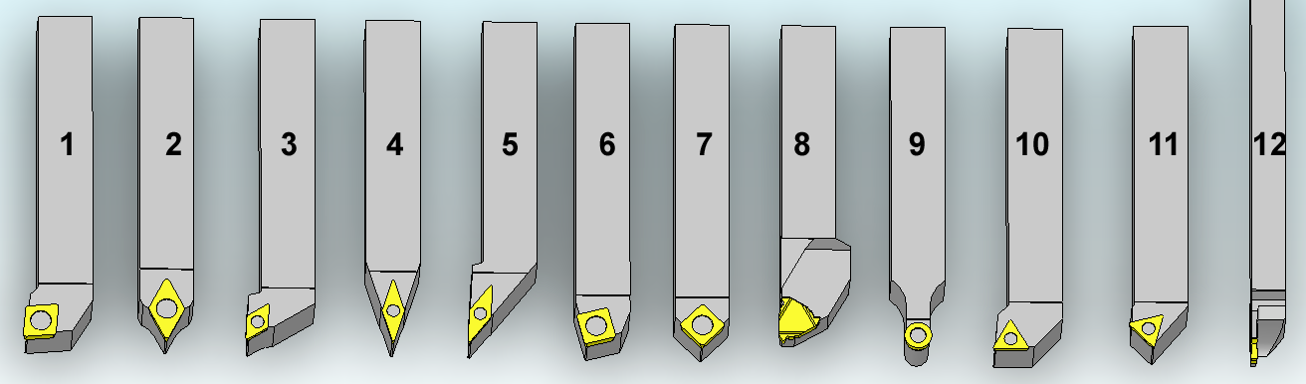
\includegraphics[width=0.8\linewidth]{img/Picture18}

~\

\begin{tabular}{|l|l|}
\hline
1 à 6 et 9 & Outils à charioter \\
\hline
7 et 11 & Outils à chanfreiner \\
\hline
8 & Outil à fileter \\
\hline
10 & Outil à dresser \\
\hline
11 & Outil à gorge ou à tronçonner\\
\hline
\end{tabular}
\end{center}
}}

{\frame{
\frametitle{Outils de fraisage}

\begin{minipage}{0.48\linewidth}
\begin{center}
 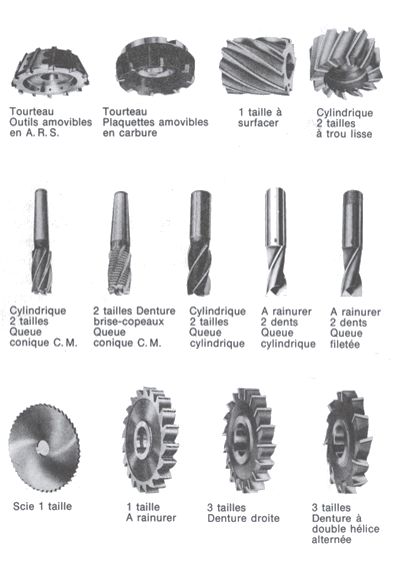
\includegraphics[width=0.9\linewidth]{img/Picture19}
\end{center}
\end{minipage}\hfill
\begin{minipage}{0.48\linewidth}
\begin{center}
 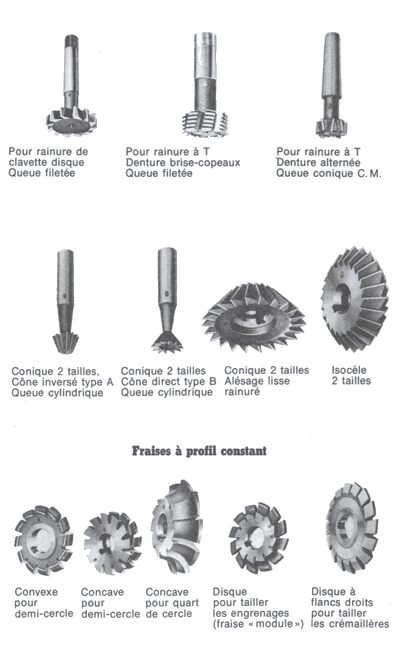
\includegraphics[width=0.8\linewidth]{img/Picture20}
\end{center}
\end{minipage}
}}

{\frame{
\frametitle{Les porte-pièces}

\begin{itemize}
 \item Les portes-pièces permettent de maintenir la pièce sur la machine pendant les phases d'usinage, il en existe plusieurs types,
 \item La compréhension de la mise en position de la pièce sur la machine (par l'intermédiaire du porte-pièce) est impérative. Il faut tenir compte de l'isostatisme du montage.
\begin{minipage}{0.7\linewidth}
 \item \textbf{Le mandrin} : La pièce est placée entre les mors du mandrin.
Un serrage concentrique des 3 mors permet de maintenir la pièce.
Le mandrin est installé sur la machine, il est entraîné en rotation par le moteur de broche.
\end{minipage}\hfill
\begin{minipage}{0.25\linewidth}
   \begin{center}
  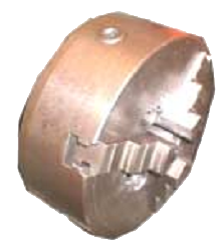
\includegraphics[width=0.9\linewidth]{img/Picture21}
  \end{center}
\end{minipage}
\end{itemize}
}}

{\frame{
\frametitle{Les porte-pièces}

\begin{itemize}
\begin{minipage}{0.7\linewidth}
 \item \textbf{L'étau} : Utilisé pour les pièces prismatiques. Ce porte pièce est composé de 2 mors. Le mors fixe est lié au bâti. Le mors mobile, en liaison glissière avec le bâti permet le serrage de la pièce. La pièce est donc placée entre les deux mors de l'étau. 
\end{minipage}\hfill
\begin{minipage}{0.25\linewidth}
   \begin{center}
  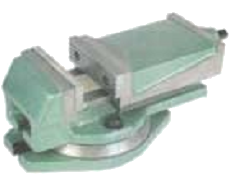
\includegraphics[width=0.9\linewidth]{img/Picture23}
  \end{center}
\end{minipage} \\ ~\ \\ ~\ \\
\begin{minipage}{0.7\linewidth}
 \item \textbf{Le montage d'usinage} : Utilisé pour les pièces complexes. Il s'appui sur une plaque percée sur laquelle il faut ajouter différents supports qui s'adaptent aux surfaces de la pièce. Les appuis doivent être définis afin de supprimer les degrés de liberté de la pièce sans hyperstatisme. La pièce est maintenue par des brides serrés par des vis.
\end{minipage}\hfill
\begin{minipage}{0.25\linewidth}
   \begin{center}
  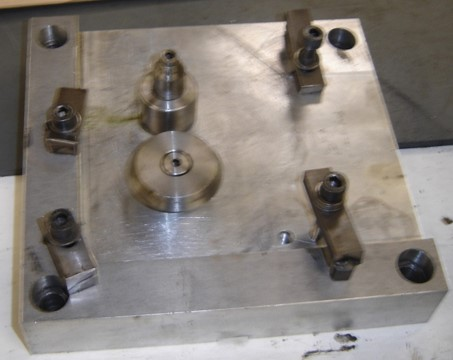
\includegraphics[width=0.9\linewidth]{img/Picture24}
  \end{center}
\end{minipage}
\end{itemize}
}}

\section{Paramètres de coupe}

\ifdef{\public}{{\frame{
\frametitle{Plan}
  \tableofcontents[currentsection]
}}}

{\frame{
\frametitle{Paramètres de coupe}

\begin{itemize}
 \item Lors d'un usinage par enlèvement de matière, on se retrouve, dans la majorité des cas, dans la configuration suivante :
 \begin{itemize}
  \item Une lame d'outil pénètre dans la matière et enlève un copeau,
  \item L'outil suit une trajectoire par rapport à la pièce à usiner,
  \item Pour obtenir un travail satisfaisant (bon état de la surface usinée, rapidité de l'usinage, usure modérée de l'outil, ...) on doit régler les paramètres de la coupe.
  \end{itemize}
\begin{minipage}{0.45\linewidth}
 \item Plusieurs critères permettent de définir les paramètres de la coupe:
 \begin{itemize}
  \item Le type de machine (tournage, fraisage, perçage),
  \item La puissance de la machine,
  \item La matière de la pièce et de l'outil,
  \item Le type de l'opération (perçage, chariotage,...),
  \end{itemize}
 \item Les paramètres sont les suivants:
 \begin{itemize}
  \item La vitesse de coupe : Vc,
  \item La vitesse d'avance : F,
  \item La profondeur de passe : a.
 \end{itemize}  
\end{minipage}\hfill
\begin{minipage}{0.5\linewidth}
   \begin{center}
  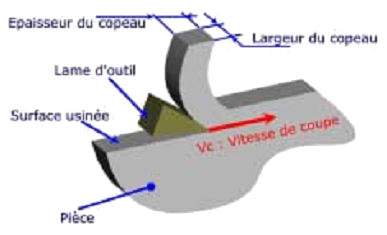
\includegraphics[width=0.8\linewidth]{img/Picture245}
  \end{center}
\end{minipage}
\end{itemize}
}}

{\frame{
\frametitle{Paramètres de coupe}

\begin{itemize}
 \item La vitesse de coupe : \textbf{Vc} $m.min^{-1}$: elle correspond au déplacement de l'arête de coupe par rapport à la pièce,
 \item La vitesse d'avance : \textbf{Vf} $mm.min^{-1}$: elle correspond à la vitesse de déplacement de l'outil sur la trajectoire d'usinage,
 \item La profondeur de passe : \textbf{a} $mm$: la combinaison de $Vf$ et $a$ permet de déterminer le volume du copeau.
\end{itemize}
}}

{\frame{
\frametitle{Paramètres de coupe: Tournage}

\begin{itemize}
 \item La vitesse de coupe : \textbf{Vc} $m.min^{-1}$: cette vitesse est donnée par la vitesse de rotation de la pièce. En prenant le diamètre D ($mm$) comme la position de la pointe de l'outil et N ($tr.min^{-1}$) la vitesse de rotation: $N=\dfrac{1000.Vc}{\pi.D}$,\\ ~\ \\
\begin{minipage}{0.55\linewidth}
 \item La vitesse d'avance : \textbf{Vf} $mm.min^{-1}$: la relation entre la vitesse d'avance, celle de rotation et $fz$ l'avance à la dent ($mm.tr^{-1}$) est la suivante: $Vf=f_z.N$, \\
\end{minipage}\hfill
\begin{minipage}{0.4\linewidth}
   \begin{center}
  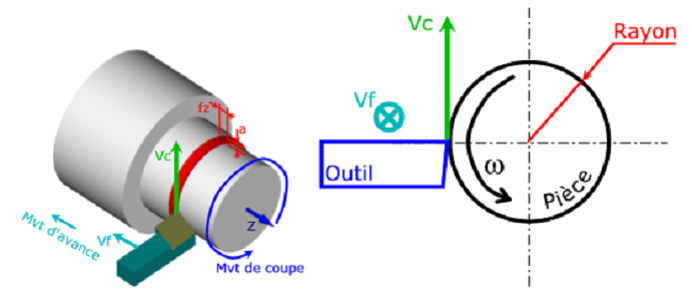
\includegraphics[width=\linewidth]{img/Picture25}
  \end{center}
\end{minipage}
 \item $fz$ correspond à la distance que l'arête de coupe va parcourir à chaque tour de la pièce.
\end{itemize}
}}

{\frame{
\frametitle{Paramètres de coupe: Fraisage}

\begin{itemize}
 \item La vitesse de coupe : \textbf{Vc} $m.min^{-1}$: cette vitesse est donnée par la vitesse de rotation de l'outil. En prenant le diamètre D ($mm$) comme le diamètre de l'outil et N ($tr.min^{-1}$) sa vitesse de rotation: $N=\dfrac{1000.Vc}{\pi.D}$,\\ ~\ \\
\begin{minipage}{0.55\linewidth}
 \item La vitesse d'avance : \textbf{Vf} $mm.min^{-1}$: la relation entre la vitesse d'avance, celle de rotation et $fz$ l'avance à la dent ($mm.tr^{-1}$) est la suivante: $Vf=f_z.z.N$, \\
\end{minipage}\hfill
\begin{minipage}{0.4\linewidth}
   \begin{center}
  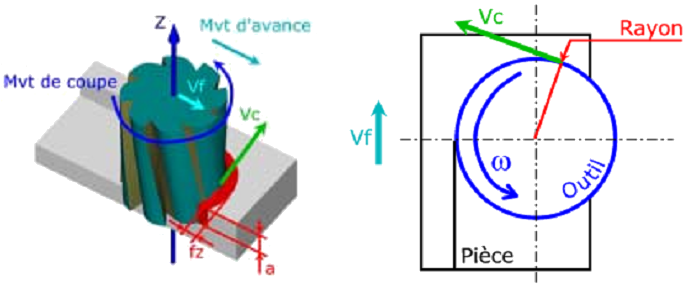
\includegraphics[width=\linewidth]{img/Picture255}
  \end{center}
\end{minipage}
 \item $fz$ correspond à la distance que l'arête de coupe va parcourir à chaque passage de dent sur la pièce.
\end{itemize}
}}

\section{Processus}

\ifdef{\public}{{\frame{
\frametitle{Plan}
  \tableofcontents[currentsection]
}}}

{\frame{
\frametitle{Mise en position de la pièce (MIP)}

~\

\begin{minipage}{0.45\linewidth}
\begin{itemize}
 \item Pour immobiliser un solide, il faut supprimer 6 degrés de liberté,
 \item Le placement doit être isostatique,
 \item \textit{Exemple}: percer un trou respectant les cotes A et B.
\end{itemize}
\end{minipage}\hfill
\begin{minipage}{0.5\linewidth}
   \begin{center}
  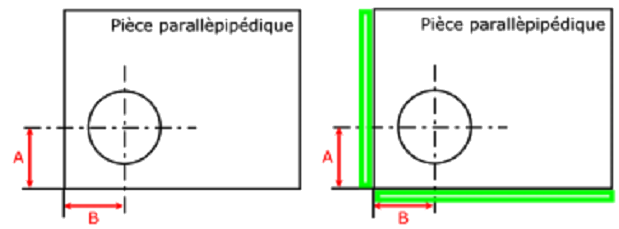
\includegraphics[width=0.9\linewidth]{img/Picture26}
  \end{center}
\end{minipage}

   \begin{flushleft}
  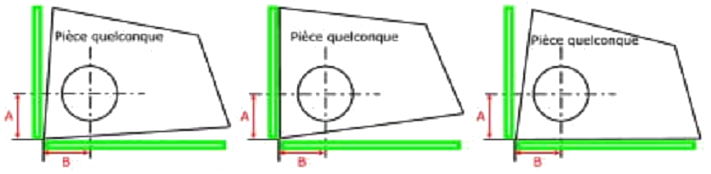
\includegraphics[width=0.7\linewidth]{img/Picture27}
  \end{flushleft}
  
     \begin{flushright}
  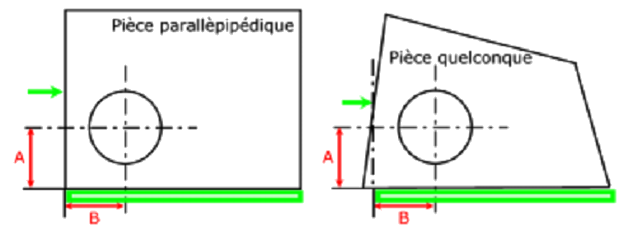
\includegraphics[width=0.45\linewidth]{img/Picture28}
  \end{flushright}
}}

{\frame{
\frametitle{Mise en position de la pièce (MIP)}

\begin{minipage}[t]{0.4\linewidth}
\begin{itemize}
 \item Associer plusieurs liaisons simples permet de supprimer les 6 degrés de liberté,
 \item A partir de la le concept de centrage long ou court favorise plus ou moins certains de ces contacts.
\end{itemize}
\end{minipage}\hfill
\begin{minipage}[t]{0.5\linewidth}
~\ \\
  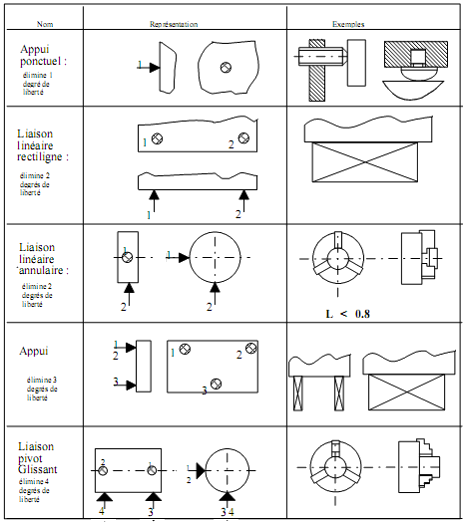
\includegraphics[width=0.9\linewidth]{img/Picture29}
\end{minipage}
}}

{\frame{
\frametitle{Gammes de fabrication}

\begin{itemize}
 \item \textbf{Opération d'usinage} : fait de réaliser l'usinage d'une surface sur une pièce (dressage, chariotage, perçage, surfaçage,...),
 \item \textbf{Phase d'usinage} : regroupement d'une ou plusieurs opérations réalisées sur la pièce. La mise en position sera unique, et la pièce ne DOIT PAS être démonte entre les opérations. On change de phase à chaque démontage de pièce,
 \item \textbf{Contrat de phase} : document qui décrit la phase d'usinage,
 \item \textbf{Gamme d'usinage} : regroupement de l'ensemble des phases d'usinage, 
 \item \textbf{Gamme d'usinage} : document qui décrit la méthode complète d'obtention de la pièce.
\end{itemize}
}}

{\frame{
\frametitle{Gammes d'usinage}

\begin{itemize}
 \item Afin d'améliorer la fabrication d'une pièce, il faut minimiser le nombre de phases d'usinage,
 \item C'est pour cela que sur chaque phase, il faut viser à maximiser le nombre de surfaces usinées.
 \item Usiner deux surfaces dans la même phase permet de minimiser les défauts de position relatifs. Ainsi, ce sont les spécifications qui décident de la gamme d'usinage.
\end{itemize}
}}

{\frame{
\frametitle{Gammes d'usinage}

\begin{center}
 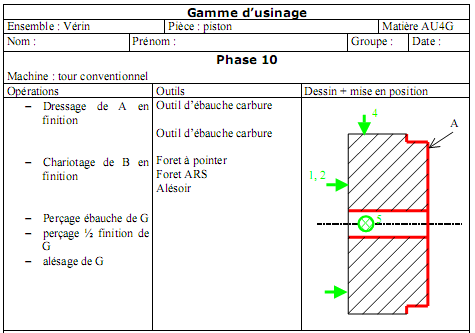
\includegraphics[width=0.9\linewidth]{img/Picture301}
\end{center}
}}

{\frame{
\frametitle{Gammes d'usinage}

\begin{center}
 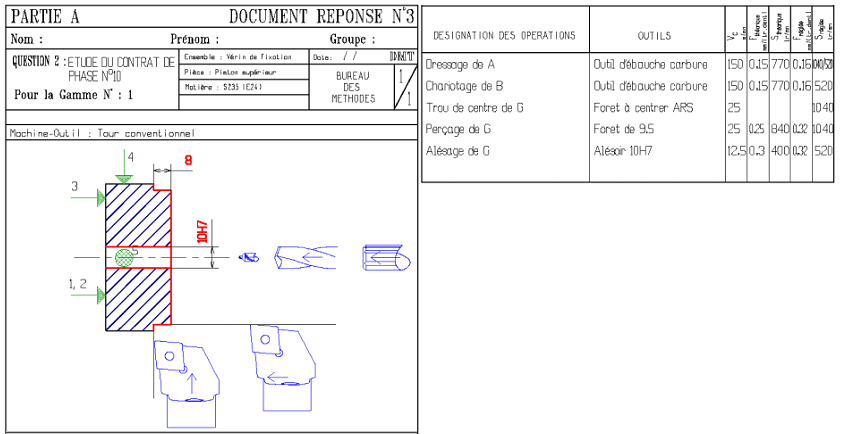
\includegraphics[width=\linewidth]{img/Picture311}
\end{center}
}}

{\frame{
\frametitle{Conclusion}

\begin{savoir}
Vous êtes capables :
\begin{itemize}
 \item de concevoir une pièce usinée,
 \item de décrire le processus d'usinage.
\end{itemize}
\end{savoir}
\vfill
}}

\end{document}